\documentclass[table]{beamer}
\usetheme{ttuStatsCamp}
%\usefonttheme{serif}
\usepackage[T1]{fontenc}
\usepackage[utf8]{inputenc}
\usepackage{mathptmx}
\usepackage{url}
\usepackage{graphicx}
\usepackage{setspace}
\usepackage{esint}
\usepackage[natbibapa]{apacite}
%\usepackage{color}
\usepackage{amsmath}
\usepackage{amsfonts}
\usepackage{bm}
\usepackage{Sweavel}
\usepackage{listings}

\def\Sweavesize{\scriptsize}
\def\Rcolor{\color{black}}
\def\Routcolor{\color{black}}
\def\Rcommentcolor{\color{violet}}
\def\Rbackground{\color[gray]{0.85}}
\def\Routbackground{\color[gray]{0.85}}

\lstset{tabsize=2, breaklines=true, style=Rstyle}



\newcommand{\red}[0]{\textcolor{red}}
%\newcommand{\violet}[0]{\textcolor{violet}}
\newcommand{\green}[0]{\textcolor{green}}
\newcommand{\blue}[0]{\textcolor{blue}}
\newcommand{\comment}[1]{}
\newcommand{\kfold}[0]{\emph{K}-fold cross-validation}

\title{Univariate Multiple Imputation}

\author{Kyle M. Lang \& Todd D. Little}

\institute[TTU IMMAP]{
  Institute for Measurement, Methodology, Analysis \& Policy\\
  Texas Tech University\\
  Lubbock, TX
}

\date{November 6, 2015}


\begin{document}

\setkeys{Gin}{width=\textwidth}
  
\input{sweaveFiles/lecture2-001}


\begin{frame}[plain]
  
  \titlepage
  
\end{frame}


\begin{frame}{Outline}
  
  \begin{itemize}
  \item Look at MI in more depth
    \vspace{12pt}
    \begin{itemize}
    \item Build up a basis of MI by starting from ordinary least
      squares regression.
    \item Demonstrate each step with examples in \textsf{R}.
    \item Show how to manually implement a simple MI in \textsf{R}.
    \end{itemize}
  \end{itemize}
  
\end{frame}


\begin{frame}[shrink = 5]{Levels of Uncertainty Modeling}

  \citet{vanBuuren:2012} provides a very useful classification of different imputation methods:
  \vspace{12pt}
  \begin{enumerate}
  \item Simple Prediction.
    \begin{itemize}
    \item The missing data are naively filled with predicted values from some regression equation.
    \item All uncertainty is ignored
    \end{itemize}
    \vspace{12pt}
  \item Prediction + Noise
    \begin{itemize}
    \item A random residual error is added to each predicted value to create the imputations
    \item Only uncertainty in the predicted values is modeled
    \item The imputation model itself is assumed to be correct and error-free
    \end{itemize}
    \vspace{12pt}
  \item Prediction + Noise + Model Error
    \begin{itemize}
    \item Uncertainty in the imputation model itself is also modeled
    \item Only way to get fully proper imputations in the sense of \citet{rubin:1987}.
    \end{itemize}
  \end{enumerate}
  
\end{frame}


\begin{frame}[shrink = 5]{Do we really need to worry?}

  The arguments against single imputation can seem archaic and
  petty. Do we really need to worry about this stuff?\\  
  \pause
  \vspace{12pt}
  YES!!!\\
  \vspace{12pt}
  The following are results from a simple Monte Carlo simulation:
  
% latex table generated in R 3.2.2 by xtable 1.7-4 package
% Thu Nov  5 15:44:16 2015
\begin{table}[ht]
\centering
\scalebox{0.8}{
\begin{tabular}{|r|c|c|c|c|}
  \rowcolor{white}  \hline
 & Complete Data & Conditional Mean & Stochastic & MI \\ 
  \rowcolor{white}  \hline
cor(X, Y) & 0.500 & 0.563 & 0.498 & 0.497 \\ 
   \rowcolor{white} Type I Error & 0.052 & 0.138 & 0.120 & 0.054 \\ 
   \rowcolor{white}  \hline
\end{tabular}
}
\caption{Mean Correlation Coefficients and Type I Error Rates} 
\end{table}

\pause
\vspace{-12pt}
\begin{itemize}
\item Conditional mean substitution overestimates the correlation
  effect.
  \vspace{6pt}
\item Both single imputation methods inflate Type I error rates.
  \vspace{6pt}
\item Only MI provides unbiased point estimates and accurate Type I
  error rates.
\end{itemize}

\end{frame}


\begin{frame}{Brief Regression Refresher}
  
  Ordinary least squares (OLS) regression estimates the following
  model:
  \begin{align}
    y = \mathbf{X}\beta + \varepsilon
  \end{align}
  By minimizing the residual sum of squared errors, we get the
  following estimated regression coefficients:
  \begin{align}
     \beta = \left(\mathbf{X}^T \mathbf{X} \right)^{-1} \mathbf{X}^T y
  \end{align}
  We can predict the values of unobserved outcome data by applying the
  fitted $\beta$s to new predictor data:
  \begin{align}
    \hat{y} = \mathbf{X}_{new}\beta
  \end{align}
  These predicted values are the basis for nearly all imputation methods.
  
\end{frame}


\begin{frame}[allowframebreaks]{OLS Example}
    
\begin{Schunk}
\begin{Sinput}
 ## Create some data:
 X <- cbind(1, rnorm(100))
 trueBeta <- matrix(c(0.25, 0.5))
 y <- X %*% trueBeta + rnorm(100, 0.0, 0.1)
 x <- X[ , -1] # Remove constant column
 ## R's built-in solution:
 rFit <- lm(y ~ x)
 coef(rFit) # R's fitted coefficients
\end{Sinput}
\begin{Soutput}
(Intercept)           x 
  0.2515459   0.4961789 
\end{Soutput}
\begin{Sinput}
 ## Least squares by hand:
 beta <- solve(t(X) %*% X) %*% t(X) %*% y
 t(beta) # Our hand-fitted coefficients
\end{Sinput}
\begin{Soutput}
          [,1]      [,2]
[1,] 0.2515459 0.4961789
\end{Soutput}
\begin{Sinput}
 ## What about prediction?
 X2 <- cbind(1, rnorm(100, 2.0, 1.0))
 yHat <- X2 %*% beta
\end{Sinput}
\end{Schunk}

 
\pagebreak

\input{sweaveFiles/lecture2-004}
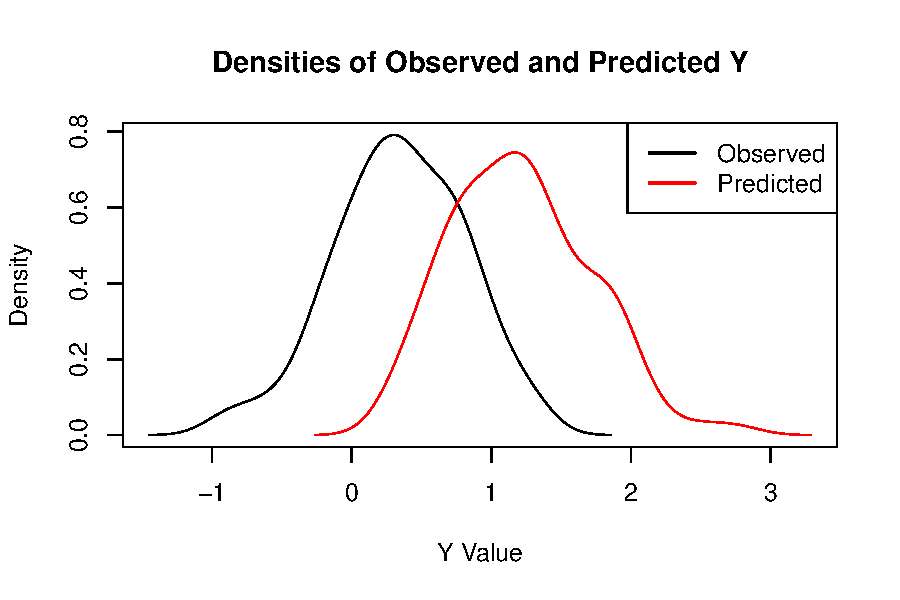
\includegraphics{sweaveFiles/lecture2-004}

\end{frame}


\begin{frame}{Simulate Some Toy Data}
  
\begin{Schunk}
\begin{Sinput}
 nObs <- 1000 # Sample Size
 pm <- 0.3 # Proportion Missing
 sigma <- matrix(c(1.0, 0.5, 0.0,
                   0.5, 1.0, 0.3,
                   0.0, 0.3, 1.0),
                 ncol = 3)
 simData <- as.data.frame(rmvnorm(nObs, c(0, 0, 0), sigma))
 colnames(simData) <- c("y", "x", "z")
 ## Impose MAR Nonresponse:
 missData <- simData
 rVec <- pnorm(missData$x,
               mean = mean(missData$x),
               sd = sd(missData$x)) < pm
 missData[rVec, "y"] <- NA
 ## Summarize and subset the data:
 nMissing <- sum(rVec)
 nObserved <- sum(!rVec)
 yMiss <- missData[rVec, ]
 yObs <- missData[!rVec, ]
 missPredData <- cbind(1, as.matrix(yMiss[ , c("x", "z")]))
 obsPredData <- cbind(1, as.matrix(yObs[ , c("x", "z")]))
\end{Sinput}
\end{Schunk}


\end{frame}


\begin{frame}{Take a look at the incomplete data}

\begin{Schunk}
\begin{Sinput}
 head(missData, n = 10)
\end{Sinput}
\begin{Soutput}
            y            x           z
1          NA -0.625895673 -1.24206938
2  -0.1448488 -0.001578954  0.47010912
3   1.2017766  1.069733846 -0.75504185
4   1.0424014 -0.192959605 -1.44583525
5   1.5970164 -0.249389277 -0.72062230
6   1.1807733  0.076461002 -3.13462011
7  -0.1738583  0.254464762  1.38601779
8  -0.4532862  1.063799386 -0.01603865
9          NA -1.712080130 -1.55090490
10  0.3816939  0.061166661 -0.15857633
\end{Soutput}
\end{Schunk}


\end{frame}


\begin{frame}{Expected imputation model parameters}
    
\begin{Schunk}
\begin{Sinput}
 ## Get the imputation model moments:
 lsFit <- lm(y ~ x + z, 
             data = missData, 
             na.action = "na.omit")
 betaHat <- matrix(coef(lsFit))
 sigma2Hat <- var(resid(lsFit))
\end{Sinput}
\end{Schunk}


\end{frame}


\begin{frame}{Conditional Mean Substitution}

\begin{Schunk}
\begin{Sinput}
 ## Get deterministic imputations:
 imp1 <- missPredData %*% betaHat
 ## Fill missing cells in Y:
 impData1 <- missData
 impData1[rVec, "y"] <- imp1
 head(impData1, n = 10)
\end{Sinput}
\begin{Soutput}
            y            x           z
1  -0.1215031 -0.625895673 -1.24206938
2  -0.1448488 -0.001578954  0.47010912
3   1.2017766  1.069733846 -0.75504185
4   1.0424014 -0.192959605 -1.44583525
5   1.5970164 -0.249389277 -0.72062230
6   1.1807733  0.076461002 -3.13462011
7  -0.1738583  0.254464762  1.38601779
8  -0.4532862  1.063799386 -0.01603865
9  -0.6766857 -1.712080130 -1.55090490
10  0.3816939  0.061166661 -0.15857633
\end{Soutput}
\end{Schunk}


\end{frame}


\begin{frame}{Stochastic Regression Imputation}
    
\begin{Schunk}
\begin{Sinput}
 ## Get stochastic imputations:
 imp2 <- missPredData %*% betaHat + 
   rnorm(nMissing, 0, sqrt(sigma2Hat))
 ## Fill missing cells in Y:
 impData2 <- missData
 impData2[rVec, "y"] <- imp2
 head(impData2, n = 10)
\end{Sinput}
\begin{Soutput}
            y            x           z
1   1.0810536 -0.625895673 -1.24206938
2  -0.1448488 -0.001578954  0.47010912
3   1.2017766  1.069733846 -0.75504185
4   1.0424014 -0.192959605 -1.44583525
5   1.5970164 -0.249389277 -0.72062230
6   1.1807733  0.076461002 -3.13462011
7  -0.1738583  0.254464762  1.38601779
8  -0.4532862  1.063799386 -0.01603865
9   0.3261248 -1.712080130 -1.55090490
10  0.3816939  0.061166661 -0.15857633
\end{Soutput}
\end{Schunk}


\end{frame}



\begin{frame}{Flavors of MI}
  
  MI simply repeats a single regression imputation $m$ times.
  \begin{itemize}
    \item The specifics of the underlying regression imputation are important, though.
  \end{itemize}
  \vspace{6pt}
  Simply repeating the stochastic regression imputation procedure described above won't suffice.
  \begin{itemize}
    \item Still produces too many Type I errors
  \end {itemize}
    
% latex table generated in R 3.2.2 by xtable 1.7-4 package
% Thu Nov  5 15:44:16 2015
\begin{table}[ht]
\centering
\scalebox{0.8}{
\begin{tabular}{|r|c|c|c|}
  \rowcolor{white} \hline
 & Complete Data & PN-Type & PNE-Type \\ 
  \rowcolor{white} \hline
cor(X, Y) & 0.499 & 0.499 & 0.498 \\ 
   \rowcolor{white}Type I Error & 0.040 & 0.066 & 0.046 \\ 
   \rowcolor{white} \hline
\end{tabular}
}
\caption{Mean Correlation Coefficients and Type I Error Rates} 
\end{table}

\vspace{-12pt}
\begin{itemize}
  \item Type I error rates for PN-Type MI are much better than they
    were for single stochastic regression imputation, but they're
    still a bit too high.
\end{itemize}

\end{frame}



\begin{frame}{Proper MI}
  
  The problems on the previous slide arise from using the same
  regression coefficients to create each of the $M$ imputations.
  \begin{itemize}
  \item Implies that you're using the ``correct'' coefficients.
    \vspace{6pt}
  \item This assumption is plainly ridiculous
    \begin{itemize}
    \item If we don't know the values of our outcome variable, how can
      we know the ``correct'' coefficients to link that unknown outcome
      to our observed predictors?
    \end{itemize}
    \vspace{6pt}
    \pause
  \item Proper MI also models uncertainty in the regression
    coefficients used to create the imputations.
    \begin{itemize}
    \item A different set of of coefficients is randomly drawn (using
      Bayesian simulation) for creating each of the $M$ imputations.
    \item The tricky part about implemented MI is deriving the
      distributions from which to sample these coefficients.
    \end{itemize}
  \end{itemize}
  
\end{frame}


\begin{frame}{Setting Up Proper MI}
  
  Our imputation model is simply a linear regression model:
  \begin{align*}
    y = \mathbf{X} \beta + \varepsilon
  \end{align*}
  To fully account for model uncertainty, we need to randomly sample
  both $\beta$ and $\text{var}(\varepsilon) = \sigma^2$.
  \begin{itemize}
  \item \textsc{Question:} Why do we only sample $\sigma^2$ and not
    $\varepsilon$?
  \end{itemize}
  \pause
  \vspace{12pt}
  For a simple imputation model with a normally distributed
  outcome and uninformative priors, we need to specifying two
  simple posterior distributions:\\
  \begin{enumerate}
    \item The marginal distribution of $\sigma^2$
    \item The conditional distribution of $\beta$ 
  \end{enumerate}
  
\end{frame}


\begin{frame}{Marginal Distribution of $\sigma^2$}
 
  We first specify the marginal posterior distribution for the noise variance $\sigma^2$.
  \begin{itemize}
  \item This distribution does not control for any other parameters.
  \end{itemize}
  \begin{align}
    \sigma^2 &\sim \text{Inv-}\chi^2 \left(N - P, s^2 \right) \label{sigma2PosteriorEq}\\
    &\text{with } s^2 = \frac{1}{N - P} \left( y - \mathbf{X}\hat{\beta}_{ls} \right)^T \left( y - \mathbf{X}\hat{\beta}_{ls} \right) \notag
  \end{align}
  \begin{itemize}
  \item $\sigma^2$ follows a scaled inverse $\chi^2$ distribution.
  \end{itemize}

\end{frame}


\begin{frame}{Conditional Distribution of $\beta$}

  We then specify the conditional posterior distribution for $\beta$. 
  \begin{itemize}
  \item This distribution is conditioned on a specific value of $\sigma^2$.
  \end{itemize}
  \begin{align}
    \beta \sim \text{MNV} \left( \hat{\beta}_{ls}, ~ \sigma^2 (\mathbf{X}^T \mathbf{X})^{-1} \right) \label{betaPosteriorEq}
  \end{align}
  \begin{itemize}
  \item $\beta$ (conditionally) follows a multivariate normal distribution.
  \end{itemize}

\end{frame}


\begin{frame}{PPD of the Missing Data}
  
  Once we've sampled our imputation model parameters as above, we can
  construct the posterior predictive distribution of the missing data.
  \begin{itemize}
    \item This is the distribution from which we sample our imputed
      values.
    \item In practice, we directly compute the imputed values based on
      the simulated imputation model parameters.
  \end{itemize}
  \begin{align}
    y_{imp} &= \mathbf{X}_{mis}\tilde{\beta} + \tilde{\varepsilon} \label{impPosteriorEq}\\
    &\text{with } \varepsilon \sim \text{N} \left( 0, \widetilde{\sigma^2} \right) \notag
  \end{align}
  
\end{frame}

  
\begin{frame}{General Steps for Basic MI}
  
  With all of the elements in place, we can execute a basic MI by
  following these steps:
  \vspace{6pt}
  \begin{enumerate}
  \item Find the least squares estimates of $\beta$,
    $\hat{\beta}_{ls}$, by regressing the observed portion of $y$
    onto the the analogous rows of $\mathbf{X}$.
    \vspace{6pt}
  \item Use $\hat{\beta}_{ls}$ to parameterize the posterior
    distribution of $\sigma^2$, given by Equation
    \ref{sigma2PosteriorEq}, and draw $M$ samples of $\sigma^2$ from
    this distribution.
    \vspace{6pt}
  \item For each of the $\sigma^2_m$, sample a corresponding value of
    $\beta$ from Equation \ref{betaPosteriorEq}.
    \vspace{6pt}
  \item Plug the $M$ samples of $\beta$ and $\sigma^2$ into Equation
    \ref{impPosteriorEq} to create the $M$ imputations.
  \end{enumerate}
  
\end{frame}


\begin{frame}{MI by Hand}
      
  First, we need to sample from the marginal posterior distribution of
  $\sigma^2$.
  
\begin{Schunk}
\begin{Sinput}
 ## Do MI by hand:
 nImps <- 100
 nSams <- 5000
 df <- nObserved - length(betaHat)
 sigmaScale <- 
   (1 / df) * crossprod(yObs$y - obsPredData %*% betaHat)
 sigmaSams <- rinvchisq(nSams, df = df, scale = sigmaScale)
\end{Sinput}
\end{Schunk}


\end{frame}


\begin{frame}{MI by Hand}
  
  Then we need to use those samples of $\sigma^2$ to parameterize the
  conditional posterior distribution of $\beta$ and sample from it.
  
\begin{Schunk}
\begin{Sinput}
 betaVarDenom <- solve(crossprod(obsPredData))
 betaSams <- matrix(NA, nSams, length(betaHat))
 for(m in 1 : nSams) {
   betaSigma <- sigmaSams[m] * betaVarDenom
   betaSams[m, ] <- 
     rmvnorm(1, mean = betaHat, sigma = betaSigma)
 }
\end{Sinput}
\end{Schunk}


\end{frame}


\begin{frame}{MI by Hand}
  
  Finally, we use the sampled imputation model moments to construct
  the missing data's posterior predictive distribution:
  
\begin{Schunk}
\begin{Sinput}
 impMat <- matrix(NA, nMissing, nSams)
 for(m in 1 : nSams) {
   impMat[ , m] <-
     missPredData %*% matrix(betaSams[m, ]) +
           rnorm(nMissing, 0, sqrt(sigmaSams[m]))
 }
 ## We wrap everything up by filling-in the missing
 ## cells in 'missData' with the M imputations
 impList <- list()
 for(m in 1 : nImps) {
   impList[[m]] <- missData
   impList[[m]][rVec, "y"] <- impMat[ , m]
 }
\end{Sinput}
\end{Schunk}


\end{frame}


\begin{frame}{What do we get?}
    
\input{sweaveFiles/lecture2-014}
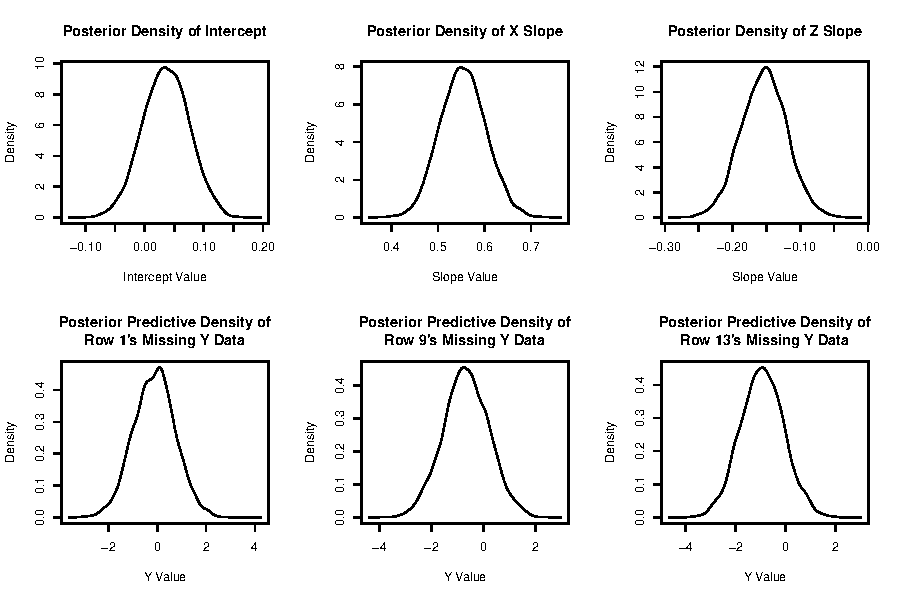
\includegraphics{sweaveFiles/lecture2-014}

\end{frame}


\begin{frame}[shrink = 5]{Doing Imputation in Practice}
  Each of the preceding approaches is available in the \textsf{R}
  package \texttt{mice} \citep{mice}.
    
\begin{Schunk}
\begin{Sinput}
 ## Conditional Mean Substitution:
 miceOut1 <- mice(missData,
                  m = 1,
                  maxit = 1,
                  method = "norm.predict",
                  printFlag = FALSE)
 impDat1 <- complete(miceOut1)
 ## Stochastic Regression Imputation:
 miceOut2 <- mice(missData,
                  m = 1,
                  maxit = 1, 
                  method = "norm.nob",
                  printFlag = FALSE)
 impDat2 <- complete(miceOut2)
 ## Proper MI:
 miceOut3 <- mice(missData,
                  m = nImps,
                  maxit = 1,
                  method = "norm",
                  printFlag = FALSE)
 impList2 <- list()
 for(m in 1 : nImps) impList2[[m]] <- complete(miceOut3, m)
 ## NOTE: Only set maxit = 1 with exactly 1 incomplete variable
\end{Sinput}
\end{Schunk}


\end{frame}


\begin{frame}[allowframebreaks]{References}

  \bibliographystyle{apacite}
  \bibliography{/home/kylelang/data/academics/literature/bibtexFiles/dissRefsList.bib}
 
\end{frame}



\end{document}
